\section{Marketing}
Marketing is the process of creating, communicating, delivering, and exchanging offerings that have value for customers, clients, partners, and society at large. It involves understanding the needs and wants of customers and creating value for them. The marketing mix consists of the 4Ps: Product, Price, Place, and Promotion.

\subsection{Evolutions in Marketing}
\begin{enumerate}
	\item \textbf{Production Era:} Focus on production and distribution efficiencies.
	\item \textbf{Product Era:} Focus on making continued product innovations.
	\item \textbf{Selling Era:} Focus on selling and promotions.
	\item \textbf{Marketing Era:} Focus on Buyer's Needs and determining the needs and wants of target markets.
\end{enumerate}
\begin{center}

	\begin{tikzpicture}[
		box/.style={draw, rectangle, minimum width=2cm, minimum height=1cm, text width=2cm, align=center},
		arrow/.style={-{Latex[length=2mm]}, thick},
		]
		
		\node[box] (driven1) at (0.2\columnwidth, 0) {Customer-\textbf{Driven}};
		\node[box] (driven2) at (0.5\columnwidth, 0) {Understand Customer Needs};
		\node[box] (driven3) at (0.8\columnwidth, 0) {Create products that meet current needs};

		\draw[arrow] (driven1) -- (driven2);
		\draw[arrow] (driven2) -- (driven3);


		\node[box] (driving1) at (0.2\columnwidth, -2) {Customer-\textbf{Driving}};
		\node[box] (driving2) at (0.5\columnwidth, -2) {Understand Customer Needs \textbf{better} than themselves};
		\node[box] (driving3) at (0.8\columnwidth, -2) {Create products that meet current \textbf{AND} future needs};

		\draw[arrow] (driving1) -- (driving2);
		\draw[arrow] (driving2) -- (driving3);
	\end{tikzpicture}
\end{center}

\subsection{Customer Relationships}
CRM is the process of building and maintaining profitable customer relationships by delivering superior customer value and satisfaction. Attracting, keeping and growing profitable customers.

\begin{center}
\begin{tikzpicture}[scale=4,
		box/.style={minimum width=2cm, minimum height=1cm, text width=2cm, align=center},
		]
    % Draw the main square
    \draw (0,0) rectangle (1,1);

    % Draw the dividing lines
    \draw (0.5,0) -- (0.5,1);
    \draw (0,0.5) -- (1,0.5);
	\scriptsize
    % Place text in each corner
	\node[box] (butterflies) at (0.25,0.75) {\textbf{Butterflies}\\Good fit between company and customer but short term};
	\node[box] (true friends) at (0.75,0.75) {\textbf{True Friends}\\Good fit between company and customer and long term};
	\node[box] (strangers) at (0.25,0.25) {\textbf{Strangers}\\Poor fit between company and customer and short term};
	\node[box] (barnacles) at (0.75,0.25) {\textbf{Barnacles}\\Poor fit between company and customer but long term};

    \node[left=0.5cm of butterflies] {High Profitability};
    \node[left=0.5cm of strangers] {Low Profitability};
    \node[above=0.5cm of butterflies] {Short Term};
    \node[above=0.5cm of true friends] {Long Term};
\end{tikzpicture}
\end{center}

\subsection{Marketing Management}
Marketing management is the art and science of choosing target markets and building profitable relationships with them. It involves planning, implementing, and controlling marketing programs to bring about exchanges with target markets to achieve organisational goals.

\begin{enumerate}
	\item \textbf{Analyse & Identify Opportunities:} Understand the marketplace and customer needs and wants.		
		\begin{itemize}
			\item Marketing Research and Information Systems
			\item Marketing Environment Scanning
			\item Consumer & Business Markets
		\end{itemize}
	\item \textbf{Research & Select Target Markets:} Find markets		
		\begin{itemize}
			\item Meassuring & Forecasting Demand
			\item Market Segmentation, Targeting, Positioning
		\end{itemize}
	\item \textbf{Design Marketing Strategies:} Develop value propositions	
		\begin{itemize}
			\item Product, Price, Place, Promotion
			\item Marketing Mix
		\end{itemize}
	\item \textbf{Managing the Marketing Effort:} Keep it working
		\begin{itemize}
			\item SWOT Analysis
			\item Planning and Objective Setting
			\item Marketing Implementation
			\item Marketing Control
		\end{itemize}
\end{enumerate}

Segmentation is dividing a market into distinct groups of buyers who have different needs, characteristics, or behaviours, and who might require separate products or marketing programs. Targeting is selecting one or more segments to enter. Positioning is the way the product is defined by consumers on important attributes and is perception based.

\section{Customer Lifetime Value}
Customer Lifetime Value (CLV) is the present value of the future cash flows attributed to the customer during his/her entire relationship with the company. It is the total revenue a company expects to earn from a customer during the entire relationship. It is important to understand the value of a customer to the company.

\subsection{Calculating CLV}
{\scriptsize \begin{align*}
	CLV &= (M-R)\left(1+\left(\frac{r}{1+d}\right)^1+\left(\frac{r}{1+d}\right)^2+\left(\frac{r}{1+d}\right)^3 + \ldots \right) \\
	&= (M-R)\left(\frac{1+d}{1+d-r}\right) \\
	&\text{If Revenue is after Service} \\
	CLV &= (M-R)\left(\frac{r}{1+d-r}\right) \\
	\text{Where:} \\
	CLV &= \text{Customer Lifetime Value} \\
	M &= \text{Margin aka Revenue} - \text{Variable Costs} \\
	R &= \text{Retention Spending} \\
	r &= \text{Retention Rate} \\
	d &= \text{Discount Rate}\\
	\text{Survival Rate} &= r^{t-1}
\end{align*}}

CLV affects the company's marketing strategy, customer acquisition, and customer retention. It is important to understand the value of a customer to the company.

Marketing should focus on the most profitable customers. The company should acquire, retain, and grow the most profitable customers. The company should also focus on customer satisfaction and loyalty. Not spend more than CLV. Remove negative CLV customers.

\subsection{Pricing}
Pricing is the process of determining what a company will receive in exchange for its products. Pricing is the only element in the marketing mix that produces revenue. All other elements represent costs. Pricing is the most flexible element of the marketing mix.

Price determines how much margin can be received from a product in relation to the relatively fixed costs of production.

\begin{center}

	\begin{tikzpicture}[
		box/.style={draw, rectangle, minimum width=2cm, minimum height=1cm, text width=4cm, align=center},
		arrow/.style={-{Latex[length=2mm]}, thick},
		]
		
		\node[box] (internal) at (0.1\columnwidth, 0) {\textbf{Internal Factors} \\ \begin{itemize} \item Organisation for Pricing \item Marketing Objectives \item Marketing Mix Strategy Costs \end{itemize}};
		\node[box] (pricing) at (0.4\columnwidth, -2) {Pricing Decisions};
		\node[box] (external) at (0.6\columnwidth, 0) {\textbf{External Factors} \\ \begin{itemize} \item Market and Demand \item Competition \item Other Environmental Concerns \end{itemize}};

		\draw[arrow] (internal) -- (pricing);
		\draw[arrow] (external) -- (pricing);

	\end{tikzpicture}
\end{center}

Costs determine the Price Floor below which the company will lose money.

Demand determines the Price Ceiling above which the company will sell nothing.

Types of Costs:
\begin{itemize}
	\item \textbf{Fixed Costs:} Costs that do not change with the level of production.
	\item \textbf{Variable Costs:} Costs that change with the level of production.
	\item \textbf{Total Costs:} Fixed Costs + Variable Costs
	\item \textbf{Average Costs:} Total Costs / Quantity
	\item \textbf{Marginal Costs:} The cost of producing one more unit.
\end{itemize}

\subsection{Experience Curve Pricing}
The experience curve is a graphical representation of the relationship between unit production costs and cumulative production quantity. The more you produce, the cheaper it gets. This is due to economies of scale, learning curve, and technological improvements.

\begin{center}
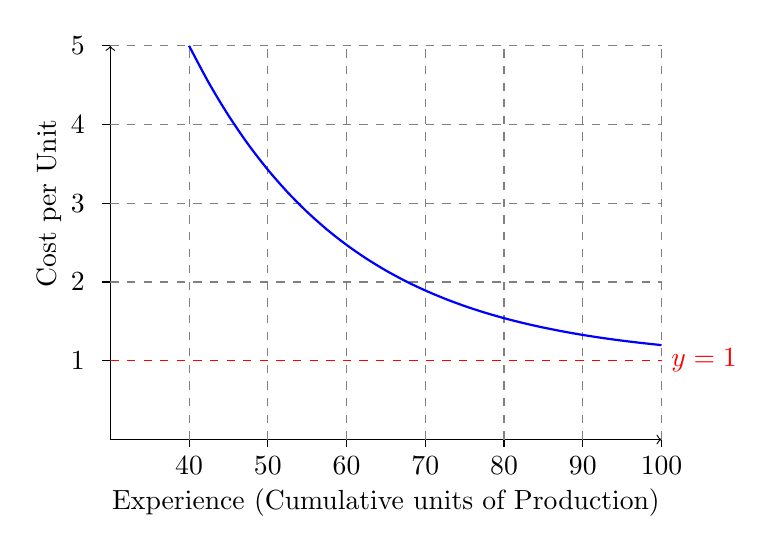
\begin{tikzpicture}
    % Define the x-axis and y-axis ranges
    \draw[->] (3,0) -- (10,0) node[below, yshift=-0.5cm, xshift=-3.5cm] {Experience (Cumulative units of Production)}; % x-axis
    \draw[->] (3,0) -- (3,5) node[left, rotate=90, anchor=south, yshift=0.5cm, xshift=-2cm] {Cost per Unit};                                % y-axis

    % Label the x-axis starting from 40
    \foreach \x in {40, 50, 60, 70, 80, 90, 100} {
        \draw (\x/10,0.1) -- (\x/10,-0.1) node[below] {\x}; % Scale x-axis to fit range
    }

    % Label the y-axis
    \foreach \y in {1, 2, 3, 4, 5} {
        \draw (2.9,\y) -- (3.1,\y) node[left, xshift=-0.3cm] {\y}; % Scale y-axis labels as needed
    }

    % Draw grid lines for x-axis and y-axis
    \foreach \x in {4, 5, 6, 7, 8, 9, 10} {
        \draw[dashed, gray] (\x,0) -- (\x,5);
    }
    \foreach \y in {1, 2, 3, 4, 5} {
        \draw[dashed, gray] (3,\y) -- (10,\y);
    }

    % Plot an example exponential decay curve (adjust as needed)
    \draw[domain=4:10, smooth, variable=\x, blue, thick] 
        plot (\x, {1 + 4*exp(-(0.5*\x-2))}); % Adjust this function as needed
    \draw[dashed, red] (3,1) -- (10,1) node[right] {$y = 1$};
\end{tikzpicture}
\end{center}

\subsection{Pricing Strategies}
\textbf{Price Skimming:} Setting a high price for a new product to skim maximum revenues layer by layer from the segments willing to pay the high price.\\
\textbf{Penetration Pricing:} Setting a low price for a new product to attract a large number of buyers and a large market share.\\
\textbf{Markup Pricing:} Adding a standard markup to the cost of the product.\\
\textbf{Target Return Pricing:} Setting the price to achieve a target return on investment.\\
$\text{Price} = \text{Direct Costs} + \frac{\text{Fixed Costs} + \text{Target Profit}}{\text{Units Sold}}$\\
\textbf{Perceived Value Pricing:} Pricing based on the perceived value of the product by the \textbf{Customer}.\\
\textbf{Psychological Pricing:} Pricing based on the psychology of the customer. E.g. \$9.99 instead of \$10\\
\textbf{Loss Leader Pricing:} Pricing a product below cost to attract customers.\\
\textbf{Captive Pricing:} Pricing the main product low and the accessories high.\\
\textbf{Product Bundle Pricing:} Pricing a bundle of products together.\\
\textbf{Price Discrimination:} Charging different prices to different customers. E.g. Senior and Student prices.\\
